
\section{Data Plane Properties}
In this section, we discuss three data plane properties and the mechanisms that support them atop the control logic. \amy{the data plane is technically below the control logic. Maybe find another word for ``atop''}

\subsection{Loss-Free Update}

%In the migration control logic, we have the concept of ``path''; let us now only focus on data plane and see how path is reflected there.

At the data plane, there is a translation table stored in each middlebox. The \system agent accepts flows for which it has established state, rewrites the header, and forwards the flow based on the supersession-subsession mapping stored in the translation table. Moving a flow from one path to another is equivalent to updating the translation tables at the data plane to accept a flow from the new subsession(s) and reject the same flow from the old subsessions. Since there are multiple middleboxes involved in the update procedure, if the update happens in the wrong order, the translation layer may drop packets, e.g. --- if the old subsession is removed before the new subsession is fully established.


Finding the right sequence of updates for a general network is proven to be NP-complete~\cite{SWAN, zUpdate}, but for a special topology, linear in our setting (we only abstract the topology between middleboxes), we can apply the concept from network consistent update~\cite{consistentupdate, ratul}. We first ensure that all new translation rules are pushed before the egress applies the new rule, and the old rules are not removed until all the new rules are installed via a complete handshake. In particular, when a migration is initialized from the middlebox (a signaling point), the middlebox notifies its neighbor through the control plane, which inserts a new rule for incoming traffic. Then this neighbor notifies the other side of the connection with an UPDATE-SYN control message. Every hop that receives UPDATE-SYN updates its own translation table. Hence once the other signaling endpoint receives the notification, a new rule for the flow has been installed at every hop for one direction of traffic; it is thus safe to apply the new rule for the egress. The opposite direction is set up in the same way with UPDATE-SYNACK messages. Once the new bidirectional path is built, we tear down the old path by removing the old rules. This loss-free update mechanism mirrors the control plane ``make before break'' philosophy and is in fact facilitated by the control plane design. 

 \begin{figure}[ht]
\centering
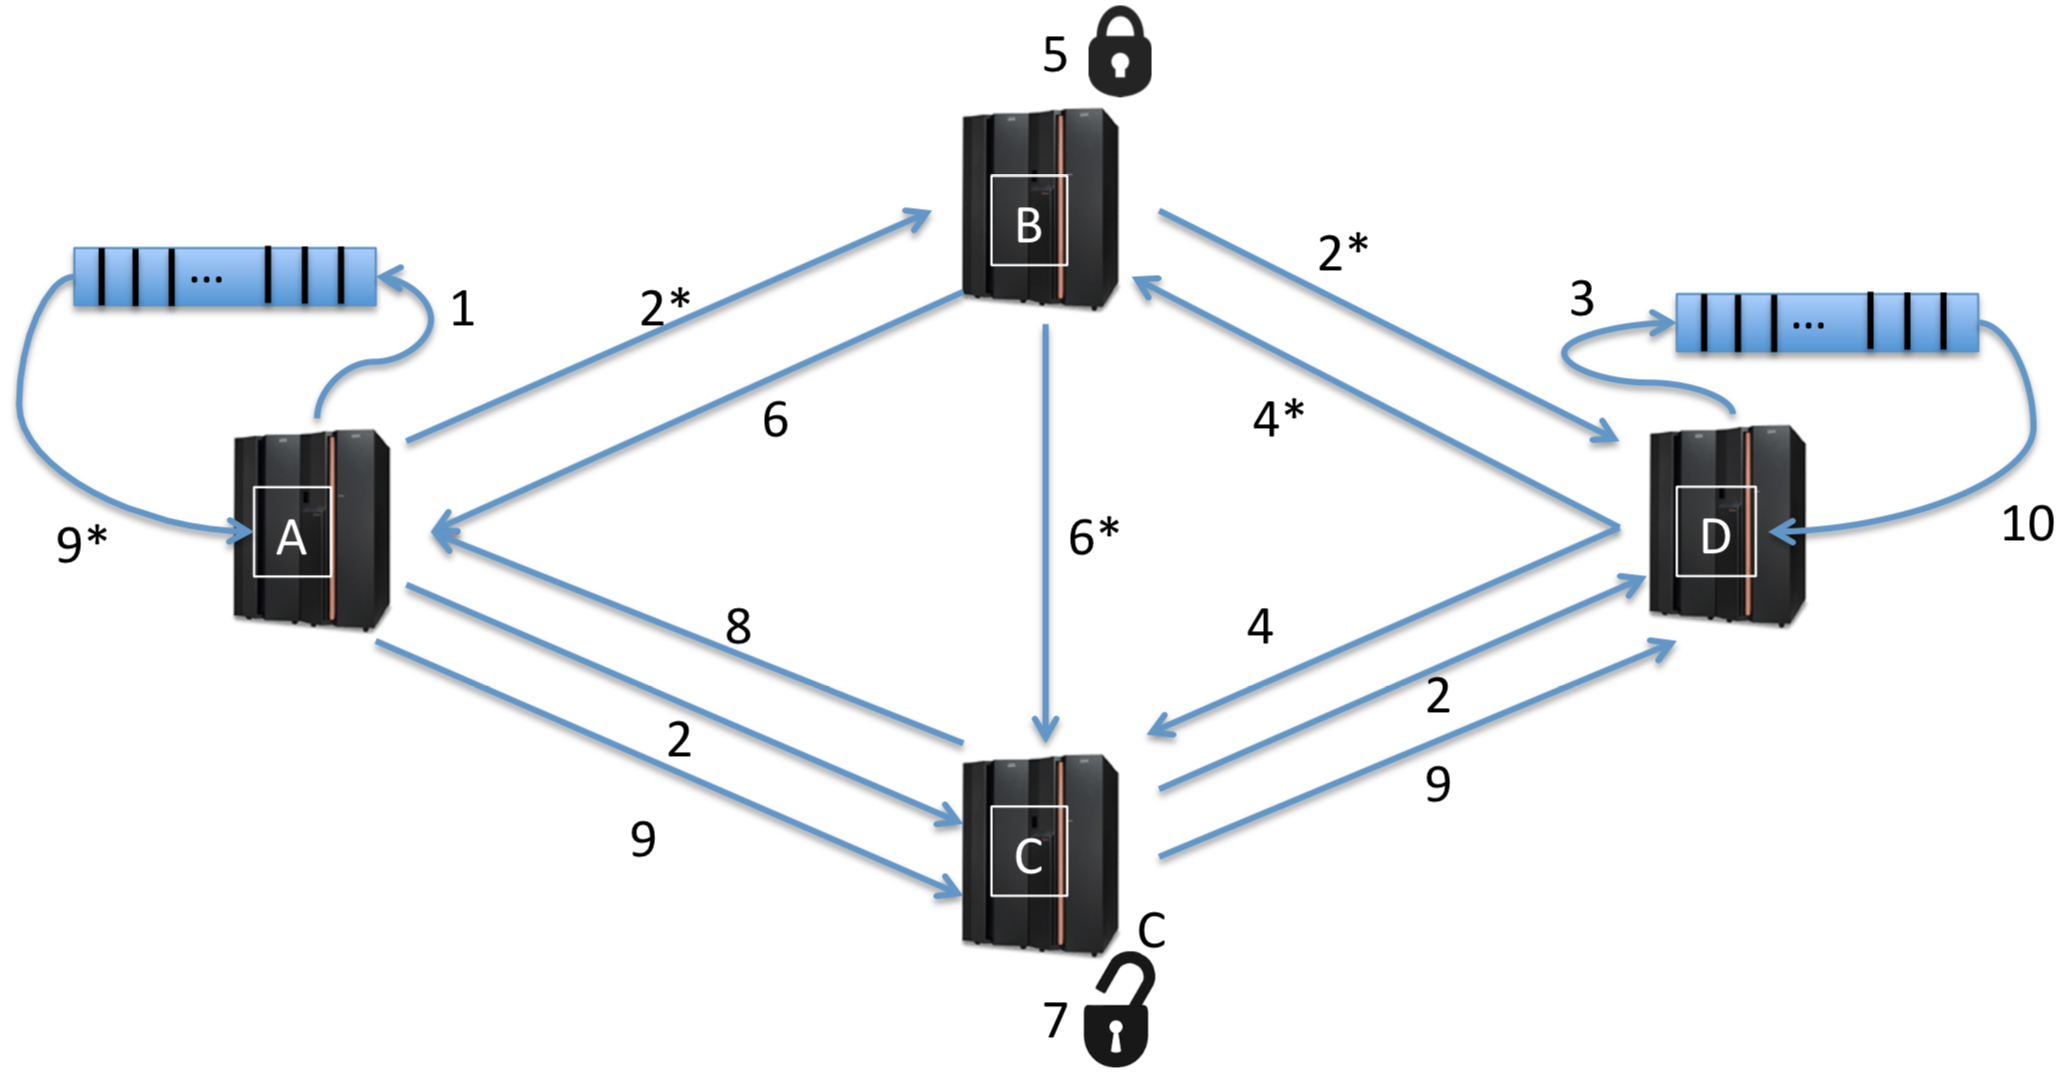
\includegraphics[width=\linewidth]{figures/order_preserving.pdf} 

\caption{Flow Migration in Packet Order Preserving ((a) and (b) can happen in parallel.)} \label{orderpreserving} 
\end{figure}
 
\subsection{Packet Order Preserving} \label{FIFO}
The previously described loss-free update is insufficient if the NF instance (state) also needs to migrate. More specifically, the NF state cannot be migrated since it is being continuously updated as packets are coming in via the old path. To lock and migrate the middlebox state, \system must stop sending traffic during the new path setup. Since changing the protocols' (e.g., TCP) flow control is undesirable, we choose to buffer the traffic and do not release it until the network function state has been replicated at the new path middlebox. Since NF state replication and migration is a well solved problem~\cite{OpenNF, splitmerge, HAMbox}, we do not address this problem here. 

A complete flow and state migration takes 10 steps as depicted in Figure~\ref{orderpreserving}: 
1) lock outgoing traffic; 
2(a) send UPDATE-SYN via new path; 
2(b) send UPDATE-FIN via old path;
3) lock the reverse direction traffic;
4(a) send UPDATE-SYNACK via new path;
4(b) send UPDATE-FINACK via old path;
5) lock middlebox states;
6(a) send UPDATE-FINACK via old path;
6(b) migrate states;
7) unlock middlebox states;
8) send UPDATE-SYNACK via new path;
9(a) send ACK packets;
9(b) release buffered traffic;
10) release buffered traffic for the other direction.
\newline \amy{is this newline intentional}


\begin{figure}[ht]
\centering
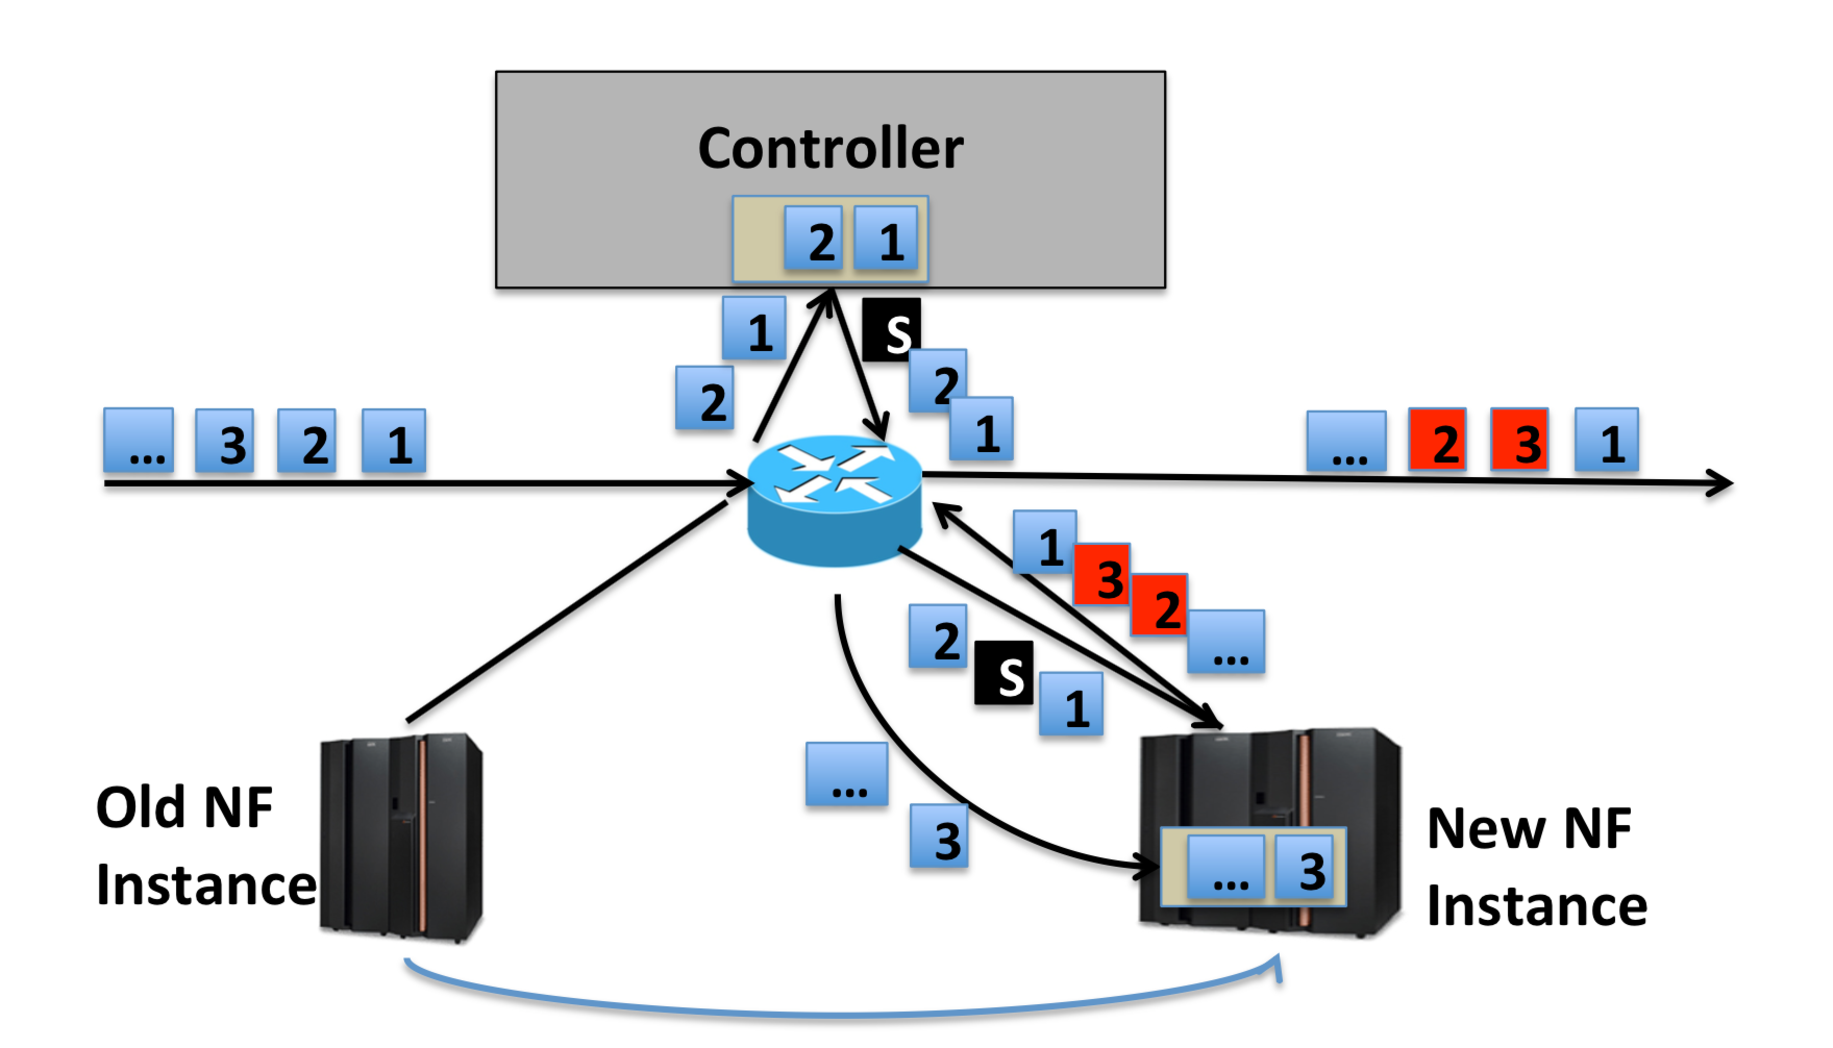
\includegraphics[width=\linewidth]{figures/opennfbroke.pdf} 
\caption{\small Order-preserving problem in OpenNF without FIFO assumption, the signal packet \texttt{s} and the data packets 1 and 2 maybe reordered and thus create reordering. Note the switch is one big switch abstraction.}\label{opennfbroke}
\end{figure}


This update mechanism also satisfies the same \textbf{packet order-preserving} property as defined in OpenNF: assuming the path with the NF instance is \textbf{FIFO}, i.e., the control message sent after the last data packet is always received after the last data packet, \textit{all packets should be processed in the order they were forwarded to the NF instance by the switch (network)}~\cite{OpenNF}. We will now show how we achieve the same property without the FIFO assumption.
 
\subsection{Substream Order Preserving}  

During migration it is useful to create two separate substreams of a byte stream (e.g., TCP), one each for the old and new path. For example, when migrating a flow from one IDS to another, we may want to ensure that all the SYNs and corresponding ACKs go through the same IDS in order to avoid an alert like ``ACK before SYN''. When the flow passes through a deep packet inspection (DPI) NF, both string matching and reg-exp matching build a Deterministic Finite Automaton (DFA), which is traversed from the root based on the byte stream~\cite{aho, yaron}. If we want to use different DPI instances for a byte stream, but the first instance has not seen a complete substream, the first DPI can only check the largest continuous byte stream before it has to buffer the remaining bytes and send them to the second DPI. 


In order to divide substreams cleanly, the left neighbor of the moving node leverages TCP sequence numbers. Suppose a migration is initiated at time $t$. The left neighbor uses the maximum seen TCP sequence number at time $t$ as a \textit{checkpoint}: it buffers packets with a higher sequence number than the checkpoint and forwards packets with a lower sequence number. \system does not lock and migrate the old NF instance state until it sees a TCP ACK with sequence number \textit{checkpoint}. The ACK guarantees the delivery of all the packets in the old substream. Note that although the buffering may create a reordering at the left neighbor middlebox, this protocol results in the correct order for the two substreams from the perspective of endpoints. See Algorithm~\ref{strictorderpres} for details. 


%%%%%%%%%%%%%%%%%%%%%%%%Algorithm %%%%%%%%%%%%%%%%%%%%%%%%%%%%%%%%%%%%%%%%%%%%
%%%%%%%%%%%%%%%%%%%%%%%%%%%%%%%%% %%%%%%%%%%%%%%%%%%%%%%%%%%%%%%%%%%%%%%%%%%%%
%%%%%%%%%%%%%%%%%%%%%%%%%%%%%%%%%  %%%%%%%%%%%%%%%%%%%%%%%%%%%%%%%%%%%%%%%%%%%%
%%%%%%%%%%%%%%%%%%%%%%%%%%%%%%%%%  %%%%%%%%%%%%%%%%%%%%%%%%%%%%%%%%%%%%%%%%%%%%
%%%%%%%%%%%%%%%%%%%%%%%%%%%%%%%%%  %%%%%%%%%%%%%%%%%%%%%%%%%%%%%%%%%%%%%%%%%%%%

\begin{algorithm} [htbp]
\footnotesize
\SetAlgoLined
\SetKwFunction{syn}{recv\_SYN}\SetKwFunction{ack}{recv\_ACK}\SetKwFunction{queue}{release\_queue}
\SetKwProg{mypacket}{Event\_Handler}{}{}
\SetKwProg{func}{Program}{}{}

\mypacket{\syn{TCP\_packet p} } {
checkpoint = hash\_lookup(p)\;
\If{p.seq $>$ checkpoint} {
Buffer (p)\;
} 
\Else{Forward(p)\;}
} 


\mypacket{\ack{TCP\_packet p}}{
\If{p.ack $>$checkpoint}{
Migrate NF state\;
//wait until migration finishes\;
sendto(left neighbor, release\_buffer)\;
}
}


\mypacket{\queue{}}{
\While{!buffer.empty()}{
Forward(buffer.dequeue())\;
}
Reset(hash\_table)\;
}

\caption{Substream Order Preserving} \label{strictorderpres}
\end{algorithm} 


%%%%%%%%%%%%%%%%%%%%%%%%Algorithm %%%%%%%%%%%%%%%%%%%%%%%%%%%%%%%%%%%%%%%%%%%%
%%%%%%%%%%%%%%%%%%%%%%%%%%%%%%%%% %%%%%%%%%%%%%%%%%%%%%%%%%%%%%%%%%%%%%%%%%%%%
%%%%%%%%%%%%%%%%%%%%%%%%%%%%%%%%%  %%%%%%%%%%%%%%%%%%%%%%%%%%%%%%%%%%%%%%%%%%%%
%%%%%%%%%%%%%%%%%%%%%%%%%%%%%%%%%  %%%%%%%%%%%%%%%%%%%%%%%%%%%%%%%%%%%%%%%%%%%%
%%%%%%%%%%%%%%%%%%%%%%%%%%%%%%%%%  %%%%%%%%%%%%%%%%%%%%%%%%%%%%%%%%%%%%%%%%%%%%


A combination of order preserving and substream separation provides us with a stronger \textbf{substream order preserving} property during an update: \textit{substreams should be processed by different NF instances in the order they were sent from the sender}. OpenNF cannot guarantee order preserving with respect to a byte stream when network links are not FIFO~\footnote{OpenNF tech report relies on this assumption in its proof.}. Furthermore, because OpenNF is by design router-based, it simply \textit{cannot} achieve substream order preserving; see Figure~\ref{opennfbroke}. Our protocol is able to provide this property precisely because the system architecture is designed to be aware of and rely on transport protocols.


Note that we may need to split the packets in the case of SYN-ACK piggyback and packet coalescing. In the first case, both directions asking for substream separation can result in deadlock since \system may choose the new path for a substream with higher sequence number in one direction and the old path for ACK as it is ACK-ing a substream with lower sequence number in the reverse direction. In the second case, the TCP client may coalesce packets, causing the payload  to cross the \textit{checkpoint} boundary in the byte stream if retransmission occurs. 







